\documentclass[conference]{IEEEtran}
\IEEEoverridecommandlockouts

\usepackage{cite}
\usepackage{amsmath,amssymb,amsfonts}
\usepackage{graphicx}
\usepackage{textcomp}
\usepackage{xcolor}
\usepackage{url}
\usepackage{booktabs}
\usepackage{multirow}

\makeatletter
\newcommand{\linebreakand}{%
  \end{@IEEEauthorhalign}
  \hfill\mbox{}\par
  \mbox{}\hfill\begin{@IEEEauthorhalign}
}
\makeatother
\begin{document}

\title{Attention Mechanisms for Theory of Mind: Weak Brain-Transformer Alignment Despite Behavioral Success}

\author{\IEEEauthorblockN{Xiaoyan Li}
\IEEEauthorblockA{\textit{Dept. of Computational Mathematics,} \\
\textit{Science and Engineering} \\
\textit{Michigan State University}\\
East Lansing, MI, USA \\
lixiaoy5@msu.edu}
\and
\IEEEauthorblockN{Cuicui Jiang}
\IEEEauthorblockA{\textit{College of Computer Science} \\
\textit{Inner Mongolia University}\\
Hohhot, China \\
jiangcuicui@mail.imu.edu.cn}
\and
\IEEEauthorblockN{Jiaoping Chen\textsuperscript{*}}
\IEEEauthorblockA{\textit{Merrick School of Business} \\
\textit{University of Baltimore}\\
Baltimore, MD, USA \\
jchen@ubalt.edu}
\linebreakand
\IEEEauthorblockN{Rumei Yang}
\IEEEauthorblockA{\textit{School of Nursing} \\
\textit{Nanjing Medical University}\\
Nanjing, China \\
rumeiyang@njmu.edu.cn}
\and
\IEEEauthorblockN{Xingyue Liu}
\IEEEauthorblockA{\textit{School of Artificial Intelligence} \\
\textit{Taiyuan University of Technology}\\
Jinzhong, China \\
2023002320@link.tyut.edu.cn}
\and
\IEEEauthorblockN{Jiaxuan Wei}
\IEEEauthorblockA{\textit{School of Artificial Intelligence} \\
\textit{Taiyuan University of Technology}\\
Jinzhong, China \\
2023002323@link.tyut.edu.cn}
}

\maketitle

% Corresponding-author note at the bottom of the first (left) column
{\renewcommand{\thefootnote}{}\footnotetext{\textsuperscript{*}Corresponding author: Jiaoping Chen (jchen@ubalt.edu).}}

\begin{abstract}
Theory of Mind (ToM), the capacity to attribute mental states to others, provides a critical test for evaluating whether language models develop genuine social understanding. We compared ToM processing in human brains (N=58, fMRI) and four transformer models (355M--7B parameters) using a modality-matched paradigm: participants listened to social versus physical descriptions of the same animated shapes, while models processed identical text transcripts. Behaviorally, 7B models achieved $75$--$83\%$ accuracy on classic ToM items (false belief, faux pas, intention), while GPT-2 variants hovered near $50\%$. Linear probes separated social from physical narrative content in model hidden states (89--98\% accuracy, versus 74\% for a bag-of-words baseline), and causal attention-head ablation identified individual heads with large effects on mental-state word prediction, although the top-5\% head set was only partly stable across 19 narrative-derived prompts. However, time-resolved encoding models produced weak brain-transformer alignment (best $r = 0.047$ in mPFC, about 19\% of the noise-ceiling upper bound); no best-layer encoding survived Benjamini--Hochberg FDR correction under unbiased layer selection, and alignment stayed weak across hemodynamic lags, nonlinear encoders and smaller ROIs. Social narratives yielded numerically higher encoding in 86\% of model$\times$layer$\times$ROI contrasts, but none of the 792 contrasts survived FDR correction, while the brain itself showed a clear voxel-wise fronto-temporal pattern for social $>$ physical processing. Attention was reliably, though only slightly, sparser for social narratives (paired tests across layers). These findings point to a dissociation between behavioral competence and representational alignment: current transformers pass ToM behavioral tests yet process social content through mechanisms that weakly align with human neural representations, suggesting fundamentally different computational strategies for social cognition. Code is publicly available at \url{https://github.com/xiaoyanLi629/attention-tom-brain-transformer}.
\end{abstract}

\begin{IEEEkeywords}
Theory of Mind, brain-transformer alignment, encoding models, fMRI, attention mechanisms, social cognition
\end{IEEEkeywords}

\section{Introduction}

Theory of Mind (ToM), the capacity to attribute mental states (beliefs, desires, intentions) to oneself and others, is fundamental to human social cognition, enabling us to navigate complex social interactions (inferring a friend's disappointment from subtle cues, predicting how colleagues will respond to unexpected news). Understanding the computational and neural mechanisms supporting ToM has been a central goal of cognitive science, with implications for developmental psychology, clinical neuroscience, and artificial intelligence \cite{frith2006neural, saxe2013people}.

Neuroscience research has identified a specialized network of brain regions supporting ToM processing. The temporoparietal junction (TPJ), particularly in the right hemisphere, shows selective activation during mental state attribution tasks \cite{saxe2013people, strachan2024testing}. Recent meta-analyses confirm that TPJ stimulation causally affects the ability to distinguish between one's own and others' mental states \cite{soutschek2025causal}. The medial prefrontal cortex (mPFC) contributes to self-other distinction \cite{amodio2006meeting}, while the posterior superior temporal sulcus (pSTS) processes biological motion and intentional action \cite{allison2000social}. Together, these regions form a ``social brain network'' \cite{mar2011neural} supporting rapid, efficient mentalizing.

Recent advances in large language models (LLMs) have raised questions about whether artificial systems can develop ToM-like capabilities. Kosinski \cite{kosinski2024evaluating} reported that GPT-3.5 and GPT-4 successfully solved classic false-belief tasks, while subsequent studies have shown mixed results depending on task modifications \cite{ullman2023large, shapira2024clever}. Recent systematic evaluations show that while GPT-4 excels at identifying indirect requests and false beliefs, it struggles with faux pas detection and lags behind humans in overall ToM performance \cite{strachan2024testing, chen2024tombench}. Furthermore, perspective-taking strategies can improve LLM ToM capabilities, suggesting that these abilities may be elicited rather than inherently present \cite{wilf2024think}. This raises a fundamental question: do LLMs genuinely understand mental states, or do they merely simulate ToM-like behavior through surface-level pattern matching? Answering this question requires examining not just behavioral performance, but the internal mechanisms underlying such performance \cite{sap2022neural, marcus2023large}. The question also matters beyond language: transformer foundation models and LLMs are increasingly used to analyze biological data, from co-assayed single-cell RNA and protein profiles \cite{ji2026captain} to cell--cell communication in single-cell and spatially resolved transcriptomics \cite{ji2024spaccc, ji2024scdca}, and interpreting such models likewise depends on knowing what their internal representations do and do not capture.

Determining whether transformers genuinely understand ToM requires complementary levels of analysis: at the \textit{structural} level, encoding models and representational similarity compare stimulus representations across biological and artificial systems \cite{kriegeskorte2008representational}, an approach established in vision \cite{khaligh2014deep} and language \cite{schrimpf2021neural, caucheteux2022brains, goldstein2022shared} but not yet applied to social cognition with modality-matched stimuli; at the \textit{content} level, probing classifiers test what is linearly decodable from hidden states \cite{elhage2021mathematical}; and at the \textit{process} level, attention sparsity and head ablation ask whether processing is concentrated in specialized components \cite{wang2022interpretability, conmy2023towards}.

A key methodological challenge in prior work has been the modality mismatch between human neuroimaging tasks and LLM inputs. Studies comparing video-based fMRI tasks with text-based LLM inputs confound modality differences with representational differences. We address this challenge by using the ``Narratives'' fMRI dataset \cite{nastase2021narratives}, where participants listened to spoken descriptions of animated shapes, one describing social interactions and another describing the same animation in purely physical terms. By feeding the identical transcripts to transformer models, we achieve modality-matched comparison, enabling a cleaner test of brain-model alignment.

We ask, at increasing mechanistic depth, whether transformer language models (1) solve classic behavioral ToM items, (2) internally distinguish ToM content from matched physical descriptions, (3) align with human brain activity during the same narratives, and (4) process social narratives through distinct attention patterns and causally necessary heads; we also ask (5) how these properties scale with model size.

\section{Related Work}

\textit{ToM in language models.} Behavioral evaluations disagree. Kosinski \cite{kosinski2024evaluating} reported near-human accuracy on false-belief tasks, but minor perturbations (e.g., transparent containers) reliably break this performance \cite{ullman2023large}, and large-scale evaluations \cite{strachan2024testing, chen2024tombench} place GPT-4 near human level on indirect requests and false belief but well below on faux pas and second-order tasks. That perspective-taking prompts boost performance \cite{wilf2024think} suggests the abilities are \emph{elicited} rather than \emph{inherent}; behavioral results alone cannot separate mental-state inference from lexical pattern matching \cite{sap2022neural, marcus2023large}.

\textit{Brain-model alignment.} Deep networks align with human visual \cite{khaligh2014deep} and language cortex \cite{schrimpf2021neural, caucheteux2022brains, goldstein2022shared}, with encoding correlations of $r=0.2$--$0.5$ (10--50\% of the ISC ceiling) typical for temporal-lobe language regions. Social cognition has received far less attention, and prior attempts often compare video-based fMRI with text-based models. The Narratives collection \cite{nastase2021narratives} enables a modality-matched comparison; its ISC ceilings in higher-order social regions are modest, which bounds the alignment one can expect.

\textit{Mechanistic interpretability.} Specific attention heads in GPT-2 implement identifiable circuits \cite{wang2022interpretability}, automated methods discover such circuits at scale \cite{conmy2023towards}, and head ablation is a standard causal test \cite{elhage2021mathematical}. Sparsity metrics such as the Gini coefficient \cite{hoyer2004non} quantify how concentrated attention is. Whether social-cognitive processing is implemented by a small identifiable circuit remains open; we test it with causal ablation (\S\ref{sec:ablation}).

\section{Methods}

\subsection{fMRI Data and Stimuli}

We used the ``Shapes'' task from the Narratives collection (OpenNeuro ds002345) \cite{nastase2021narratives}, a widely used naturalistic neuroimaging dataset. Fifty-nine participants (ages 18--35) listened to two audio narrations of the same 7-minute animated shapes film (``When Heider Met Simmel,'' copyright Yale University). The first narration was a \textit{social} description conveying intentionality and mental states (910 words), and the second was a \textit{physical} description using only geometric and motion language (951 words). For example, the social narration includes ``A young boy carrying a ball goes to an empty playground... his father shows up and calls for him... Frightened, the boy flies over the monster,'' while the physical narration describes the identical animation as ``A small triangle overlapping a smaller circle slides into a rectangle... The triangle touches the circle which glides away.'' Each participant heard both versions in a within-subject design. One participant (sub-115) was excluded due to incomplete brain coverage in posterior regions, yielding a final sample of N=58; the exclusion is applied at the subject-list level, so sub-115 is absent from every analysis, including the encoding models, the noise ceiling and the whole-brain contrast.

fMRI data were acquired on a 3T Siemens Prisma scanner at the Princeton Neuroscience Institute (TR = 1.5s, 2mm isotropic voxels, 60 slices, multiband factor 4). Each scan comprised approximately 310 volumes. The stimulus audio starts 4.5s (3 TRs) into the scan with a 37s music segment, and the narration starts at 49.5s; the first 33 TRs were trimmed, and the following 276 TRs (common to all scans) were analyzed, of which the narration occupies 272 (social) and 270 (physical) TRs.

\subsection{fMRI Preprocessing}

BOLD images were resampled from native scanner space to MNI152 standard space (2mm resolution) using nilearn's \texttt{resample\_to\_img} function with continuous interpolation. This step was critical for accurate ROI placement, as we verified that native-space affines varied by up to 44mm across subjects in the z-axis. Resampled images were spatially smoothed with a 6mm FWHM Gaussian kernel, followed by confound regression including high-pass filtering (0.01 Hz cutoff), linear detrending, and z-score normalization, implemented via nilearn's \texttt{clean\_img}.

\subsection{Regions of Interest}

ROI time series were extracted from six social brain regions defined by established meta-analytic coordinates \cite{schurz2014fractionating}: right TPJ (MNI: 54, $-$48, 24; 12mm radius), left TPJ ($-$54, $-$48, 24; 12mm), mPFC (0, 54, 18; 12mm), precuneus (0, $-$54, 36; 12mm), right STS (54, $-$42, 6; 10mm), and left STS ($-$54, $-$42, 6; 10mm). Spherical ROIs in MNI space yielded 515 voxels for the 10mm-radius STS regions and 925 voxels for the 12mm-radius ROIs. Mean time series were computed across all voxels within each ROI for each subject and condition (Fig.~\ref{fig:brain}). Because spheres of this size can straddle functional borders, we repeated the extraction and all encoding analyses with 8mm and 6mm spheres at the same centers (\S\ref{sec:robust}).

\subsection{Transformer Models}

We analyzed four transformer models spanning roughly 20$\times$ in parameter count: GPT-2-Medium (355M parameters, 24 layers, hidden size 1024), GPT-2-XL (1.5B, 48, 1600), Mistral-7B (7B, 32, 4096) and Qwen2-7B (7B, 28, 3584). Models were loaded from Hugging Face \cite{wolf2020transformers} with bfloat16 precision for the 7B models (float16 caused numerical overflow in Qwen2's logits, producing NaN outputs; bfloat16 preserves the dynamic range needed for stable forward passes) and float32 for the GPT-2 models.


\subsection{Time-Resolved Feature Extraction}
\label{sec:methods:features}

Transcripts with word-level timestamps were generated from the stimulus audio using OpenAI Whisper (small model). The dataset's canonical transcripts and forced alignments are distributed with the DataLad release of Narratives but not with the OpenNeuro snapshot we used, so we transcribed the audio directly and validated the result in two ways. First, word counts match those reported for the stimuli \cite{nastase2021narratives} (919 vs.\ 910 words for social; 943 vs.\ 951 for physical, excluding the music lyrics); second, once Whisper times are shifted by the 4.5s audio onset onto the scan clock, the first and last narration words fall at the story onset and within the story duration given in the dataset's event files, i.e.\ the narration spans exactly the 272 (social) and 270 (physical) story TRs of the official metadata. Each model read the full Whisper word sequence (music lyrics included, so that the story is processed in context) in a single forward pass. Each token was assigned to its word through character offsets (skipping the leading space that byte-level and SentencePiece tokenizers attach to word-initial tokens), each word to the TR containing its onset, and hidden states were mean-pooled over the tokens of each TR. TRs without speech (pauses) took the features of the nearest TR with speech. This produced per-layer feature matrices of shape ($n_{\text{TRs}} \times$ hidden\_dim) for each model and condition. For GPT-2 (1024-token context) the input was truncated, covering 87\% (social) and 86\% (physical) of the narration words, i.e.\ the first 89\% and 85\% of story TRs; the remaining TRs inherit the features of the last covered TR under the nearest-TR rule. We report GPT-2 encoding with these TRs included, and verified that dropping them leaves the results unchanged (\S\ref{sec:robust}).

\subsection{Encoding Models}

Ridge regression models were trained to predict each ROI's fMRI time series from LLM layer representations \cite{caucheteux2022brains, goldstein2022shared}. LLM features were shifted forward by 3 TRs (4.5s) to account for hemodynamic delay, the conventional choice given that the canonical hemodynamic response peaks 4--6s after neural activity (we test lags of 0--6 TRs in \S\ref{sec:robust}), then reduced to 50 principal components via PCA (exact SVD). Encoding performance was evaluated using Pearson $r$ between cross-validated predictions and actual time series under 5-fold temporal block cross-validation, where contiguous blocks of $\sim$55 TRs preserved temporal autocorrelation structure. This procedure was repeated for each combination of model, layer, ROI, condition, and subject (4 models $\times$ 24--48 layers $\times$ 6 ROIs $\times$ 2 conditions $\times$ 58 subjects).

The noise ceiling was estimated in the style of \cite{kriegeskorte2008representational,nastase2021narratives}. The \emph{lower bound} (a conservative reliability estimate) is the mean Pearson $r$ between each subject's time series and the average of all other subjects (leave-one-out ISC); the \emph{upper bound} is the mean correlation between each subject's time series and the grand mean across all subjects, which slightly overestimates reliability because each subject contributes to the target. Subjects with zero-variance ROI signals were excluded from both computations. Where noise-ceiling values are quoted in the text, we report the upper bound unless stated otherwise. To control for multiple comparisons across the 792 model$\times$layer$\times$ROI contrasts of social vs.\ physical encoding $r$ (paired $t$-tests across subjects), we applied Benjamini--Hochberg false-discovery-rate (FDR) correction at $q < 0.05$.

To test whether the best-layer encoding is itself above zero without the upward bias of choosing the layer on the same data, we selected the layer leave-one-subject-out: for each held-out subject, the best layer was the one with the highest mean $r$ over the other 57 subjects, and the held-out subject contributed its $r$ at that layer. The resulting 58 values were tested against zero (one-sided $t$-test, bootstrap 95\% CI), with FDR correction over the 48 model$\times$ROI$\times$condition cells.

\subsection{Whole-Brain Activation Contrast}

To visualize where in the brain social narratives drove stronger responses than physical narratives, we computed a voxel-wise group-level contrast independent of the LLM pipeline. For each of 58 subjects, preprocessed BOLD volumes (same pipeline as above) were averaged across the story-period TRs of each condition, and a subject-level difference map (social $-$ physical) was computed. Because each run is z-scored over its full length, the story-period mean expresses story activity relative to the pre-story music segment, which is identical in the two runs; the difference map is therefore (social story $-$ music) $-$ (physical story $-$ music). A one-sample $t$-test was then applied across subjects at each voxel to produce the group-level $t$-map shown in Fig.~\ref{fig:brain}A (MNI152 brain mask applied, displayed at $|t|>2.0$).

\subsection{Probing Classifiers}

For each model and layer, TR-level hidden states from both conditions were concatenated ($\sim$552 samples: 276 social + 276 physical) and classified using L2-regularized logistic regression ($C = 0.1$) with PCA reduction to 50 dimensions. Temporal block cross-validation (5-fold) was used to prevent data leakage from autocorrelation. Statistical significance was assessed via label-permutation testing (500 shuffles) at every fourth layer, with each model's best-accuracy layer additionally tested in full to obtain a reliable peak-level $p$-value. Because the two narratives differ in vocabulary (mental-state verbs vs.\ geometric terms), we ran the identical probe on bag-of-words features built from the same word-to-TR mapping, once with the full vocabulary of both narratives and once restricted to the 64 words that occur in both, i.e.\ with all condition-specific words removed.

\subsection{Attention Sparsity Analysis}

Attention sparsity was quantified per head per layer using three complementary measures. The Gini coefficient \cite{hoyer2004non}
$G = \frac{\sum_{i}\sum_{j}|a_i - a_j|}{2n\sum_i a_i}$
captures the inequality of the attention weight distribution, with $G \rightarrow 1$ indicating attention concentrated on a single token and $G = 0$ indicating uniform attention. We complement it with the normalized Shannon entropy $H = -\sum_i a_i \log_2(a_i) / \log_2(n)$, where $H \rightarrow 0$ is perfectly concentrated and $H = 1$ is uniform. A third metric, the top-5 concentration $C_5 = \sum_{i \in \text{top-5}} a_i$, directly measures the mass carried by the five most-attended tokens. A head was classified as ``sparse'' if its Gini coefficient exceeded 0.5. All three metrics were averaged across tokens, heads, layers and compared between social and physical conditions. Because heads within a layer are not independent, significance was assessed conservatively on layer means: a Wilcoxon signed-rank test over layers (social vs.\ physical, paired by layer), with effect size $d_z$ and FDR correction over models and metrics.

\subsection{Behavioral ToM Benchmark}

To complement the representational analyses, we evaluated each model on 24 classic ToM items (10 false-belief Sally--Anne items, 6 faux-pas detection items, 8 intention-attribution items). Each item consisted of a short narrative followed by a forced-choice question. For each item, we compared the model's next-token logit for the correct continuation against a single plausible distractor continuation drawn from the same narrative (e.g., ``basket'' [correct ToM prediction] vs.\ ``box'' [reality-based location]). Accuracy was the fraction of items where the correct logit exceeded the distractor; chance under this forced choice is 50\%. All logits were computed in float32 to avoid fp16 overflow on 7B models.

\subsection{Causal Head Ablation}
\label{sec:methods:ablation}

To identify which attention heads are \textit{causally} necessary for tracking social-narrative content, we ran a zero-ablation sweep on prompts derived from the social narrative, each ending just before a narrative-target word. The original set has four prompts: one character reference (\textit{father}) and three emotional states (\textit{frightened}, \textit{disappointed}, \textit{surprised}). To test the stability of the result we added 15 prompts, each a passage of the narration followed by a short frame (``The boy feels'', ``The boy is'', ``The friend wants to'') whose target is a mental-state word fitting that moment of the story (e.g.\ \textit{scared}, \textit{relieved}, \textit{lonely}, \textit{desperate}, \textit{surprise}), with a grammatical non-mental control (``the'', ``standing''); all targets are single tokens in all four tokenizers except one two-token word in Mistral. The causal effect of ablating a head was measured as the drop in logit difference between the target word and the control word (baseline minus ablated), stored per prompt. Ablation was implemented by registering a forward pre-hook on each layer's output projection (\texttt{c\_proj} for GPT-2, \texttt{o\_proj} for LLaMA/Mistral/Qwen), zeroing the corresponding head's contribution in the pre-projection tensor. ``Critical heads'' were defined as those in the top 5\% of mean ablation effects per model. Stability was quantified as the Jaccard overlap of the critical set computed on two random halves of the 19 prompts (500 splits), compared with the overlap expected for two random sets of the same size.

\section{Results}

\subsection{Behavioral ToM: Model Size Predicts Task Accuracy}
\label{sec:behavioral}

The behavioral results showed a clear scale effect (Table~\ref{tab:behavioral}). Both 7B models performed substantially above the 50\% forced-choice chance level (Qwen2-7B 83.3\% overall, Mistral-7B 75.0\%), with Qwen2-7B reaching 100\% on intention attribution and 83.3\% on faux pas. The GPT-2 variants, in contrast, performed at or below chance: GPT-2-Medium at 50.0\% overall, GPT-2-XL at 45.8\%. False belief and faux pas were the hardest categories for every model, mirroring the pattern reported in much larger models such as GPT-4 \cite{strachan2024testing}. Thus, at the behavioral level, the 7B models we study already approach competent performance on explicit ToM items. As we show below, however, these same models produce only weak alignment with human brain activity.

\begin{table}[t]
\centering
\caption{Behavioral ToM benchmark accuracy (\% correct).}
\label{tab:behavioral}
\vskip 0.05in
\begin{tabular}{lcccc}
\toprule
Model & Overall & False belief & Faux pas & Intention \\
\midrule
GPT-2-Medium & 50.0 & 40.0 & 50.0 & 62.5 \\
GPT-2-XL     & 45.8 & 40.0 & 33.3 & 62.5 \\
Mistral-7B   & 75.0 & 60.0 & 66.7 & \textbf{100.0} \\
Qwen2-7B     & \textbf{83.3} & \textbf{70.0} & \textbf{83.3} & \textbf{100.0} \\
\bottomrule
\end{tabular}
\end{table}

\subsection{Probing: LLMs Distinguish Social from Physical Content}

Linear probes classified social versus physical content from LLM hidden states well above chance (50\%) across all four models (Fig.~\ref{fig:probing}). Mistral-7B achieved the highest accuracy (98.2\%, layer 4), followed by Qwen2-7B (97.8\%, layer 4), GPT-2-Medium (94.4\%, layer 9), and GPT-2-XL (89.5\%, layer 33). The two 7B models peaked early (13--14\% relative depth) while the GPT-2 models peaked deeper (38\% and 69\%). All four peak accuracies were significant by label-permutation test: no permuted-label accuracy reached the observed value in 500 shuffles ($p < 0.002$ for every model).

Vocabulary alone already separates the conditions: a bag-of-words probe with the same pipeline reached 73.6\% ($p < 0.002$). With condition-specific words removed (64 shared words), the bag-of-words probe fell to 28.3\%, i.e.\ it carries no condition information (the below-chance value arises because the two narratives describe the same animation in the same order, so each held-out block is best matched by the temporally corresponding block of the \emph{other} condition in the training set). The LLM probes therefore exceed a purely lexical baseline by 16--25 percentage points, but part of their accuracy is lexical, and the probes are best read as showing that hidden states distinguish the two narratives, not that they encode mental-state inference as such.

\begin{figure}[t]
\centering
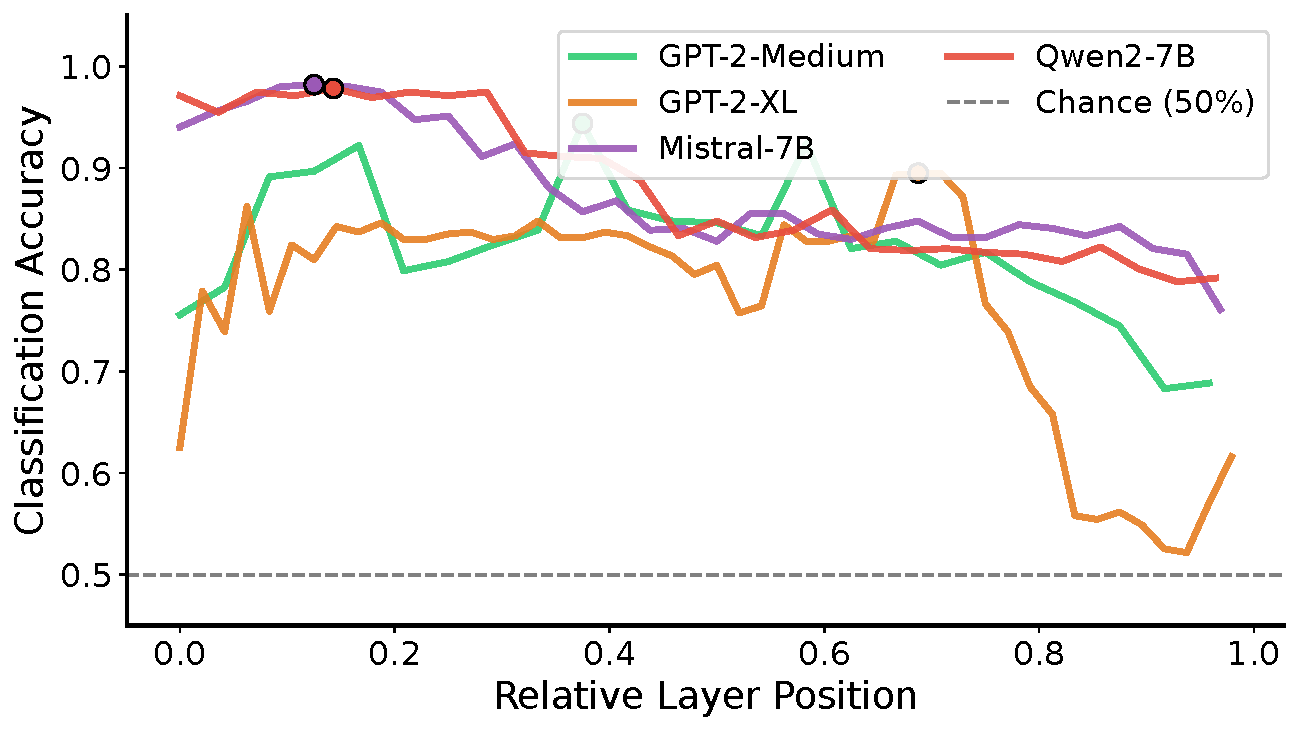
\includegraphics[width=\linewidth]{fig04_probing.pdf}
\caption{Probing accuracy for social vs.\ physical classification from LLM hidden states across relative layer position. Dashed line indicates chance (50\%); circled markers denote each model's peak layer.}
\label{fig:probing}
\end{figure}

\subsection{Encoding Models: Weak Brain-LLM Alignment}

Despite strong probing performance, time-resolved encoding models produced weak alignment between LLM representations and brain activity (Fig.~\ref{fig:encoding}). The best encoding correlations were modest: mPFC showed the strongest alignment (best $r = 0.047$, Qwen2-7B layer 19, social narrative; the other models reached 0.021--0.026), followed by lTPJ ($r = 0.034$, GPT-2-XL layer 35) and rTPJ ($r = 0.026$, Mistral-7B layer 31). These values represent about 16--21\% of the ISC-based noise-ceiling upper bound (mPFC 0.247, rTPJ and lTPJ 0.159 for the social condition). During the physical narrative no layer of any model predicted mPFC above zero (best $r$ between $-0.024$ and $-0.013$).

Even these best values are fragile. With the layer chosen leave-one-subject-out (Table~\ref{tab:encsig}), only four of the 48 model$\times$ROI$\times$condition cells exceeded zero at uncorrected $p < 0.05$, the strongest being Qwen2-7B in mPFC during the social narrative ($r = 0.047$, 95\% CI [0.018, 0.078], $p = 0.002$, 35 of 58 subjects positive), and \textbf{none survived FDR correction} (smallest $q = 0.09$). The alignment is thus weak not only relative to the noise ceiling but also in absolute terms: at the level of individual cells it cannot be reliably distinguished from zero.

\begin{table}[t]
\centering
\caption{Best-layer encoding with leave-one-subject-out layer selection (social narrative, best model per ROI; layer = group-best layer). CI: bootstrap 95\%; $q$: FDR over all 48 cells.}
\label{tab:encsig}
\vskip 0.05in
\footnotesize
\setlength{\tabcolsep}{3pt}
\begin{tabular}{llcccc}
\toprule
ROI & Model (layer) & $r$ & 95\% CI & $p$ & $q$ \\
\midrule
mPFC & Qwen2-7B (19) & 0.047 & [0.018, 0.078] & 0.002 & 0.09 \\
lTPJ & GPT-2-XL (35) & 0.029 & [0.007, 0.052] & 0.008 & 0.18 \\
rTPJ & Mistral-7B (31) & 0.026 & [0.003, 0.049] & 0.018 & 0.29 \\
PC & GPT-2-Med.\ (12) & 0.026 & [$-$0.002, 0.053] & 0.038 & 0.35 \\
lSTS & Qwen2-7B (18) & 0.025 & [$-$0.005, 0.056] & 0.057 & 0.35 \\
rSTS & Mistral-7B (31) & 0.018 & [$-$0.007, 0.042] & 0.082 & 0.36 \\
\bottomrule
\end{tabular}
\end{table}

Social narratives produced numerically stronger encoding than physical narratives in 86\% of the 792 model$\times$layer$\times$ROI contrasts, and 139 (17.6\%) reached uncorrected $p < 0.05$, all in the social $>$ physical direction and 96 of them in mPFC (Fig.~\ref{fig:enc-heatmap}). However, \textbf{none survived Benjamini--Hochberg FDR correction at $q < 0.05$} (smallest $q = 0.06$), and the mPFC effect largely reflects below-zero encoding for the physical narrative rather than strong encoding for the social one. The social advantage in alignment is therefore a consistent trend, not an established effect. A voxel-wise paired $t$-test across 58 subjects (Fig.~\ref{fig:brain}A) nevertheless recovered the expected lateral-frontal and temporal pattern for social $>$ physical processing. The five strongest positive peaks fell at MNI ($+$32, $+$20, $-$18), ($+$56, $+$2, $+$14), ($-$34, $-$8, $+$34), ($+$40, $-$88, $-$10), and ($-$46, $+$8, $+$14), corresponding broadly to right insula/orbital cortex, right superior temporal gyrus, bilateral premotor cortex, and left inferior frontal gyrus, regions consistent with agency and language-mediated social inference. The strongest negative peaks ($|t|$ up to 4.71) fell in bilateral temporal pole and cerebellum, consistent with greater motor/motion imagery during physical narratives. This confirms that the brain data themselves contain the canonical ToM signal that LLMs fail to track. The noise ceiling was highest for mPFC (lower bound 0.15--0.18, upper bound 0.23--0.25 across conditions) and lowest for bilateral STS (lower bound near zero, upper bound 0.13--0.15), indicating that inter-subject consistency varies substantially across the social brain network (Fig.~\ref{fig:brain}B). Against a circular-shift null (5000 independent rotations of each subject's series), leave-one-out ISC was significant in mPFC, precuneus and both TPJs in both conditions ($p \le 0.025$; $p < 0.001$ for mPFC), but not in STS during the social narrative ($p > 0.25$). The preprocessing therefore yields a reliable stimulus-locked signal in the regions where alignment is tested and is highest, so the weak encoding in mPFC and TPJ cannot be attributed to an unreliable ROI signal; the STS results, in contrast, are bounded by an ISC near zero.

\begin{figure}[t]
\centering
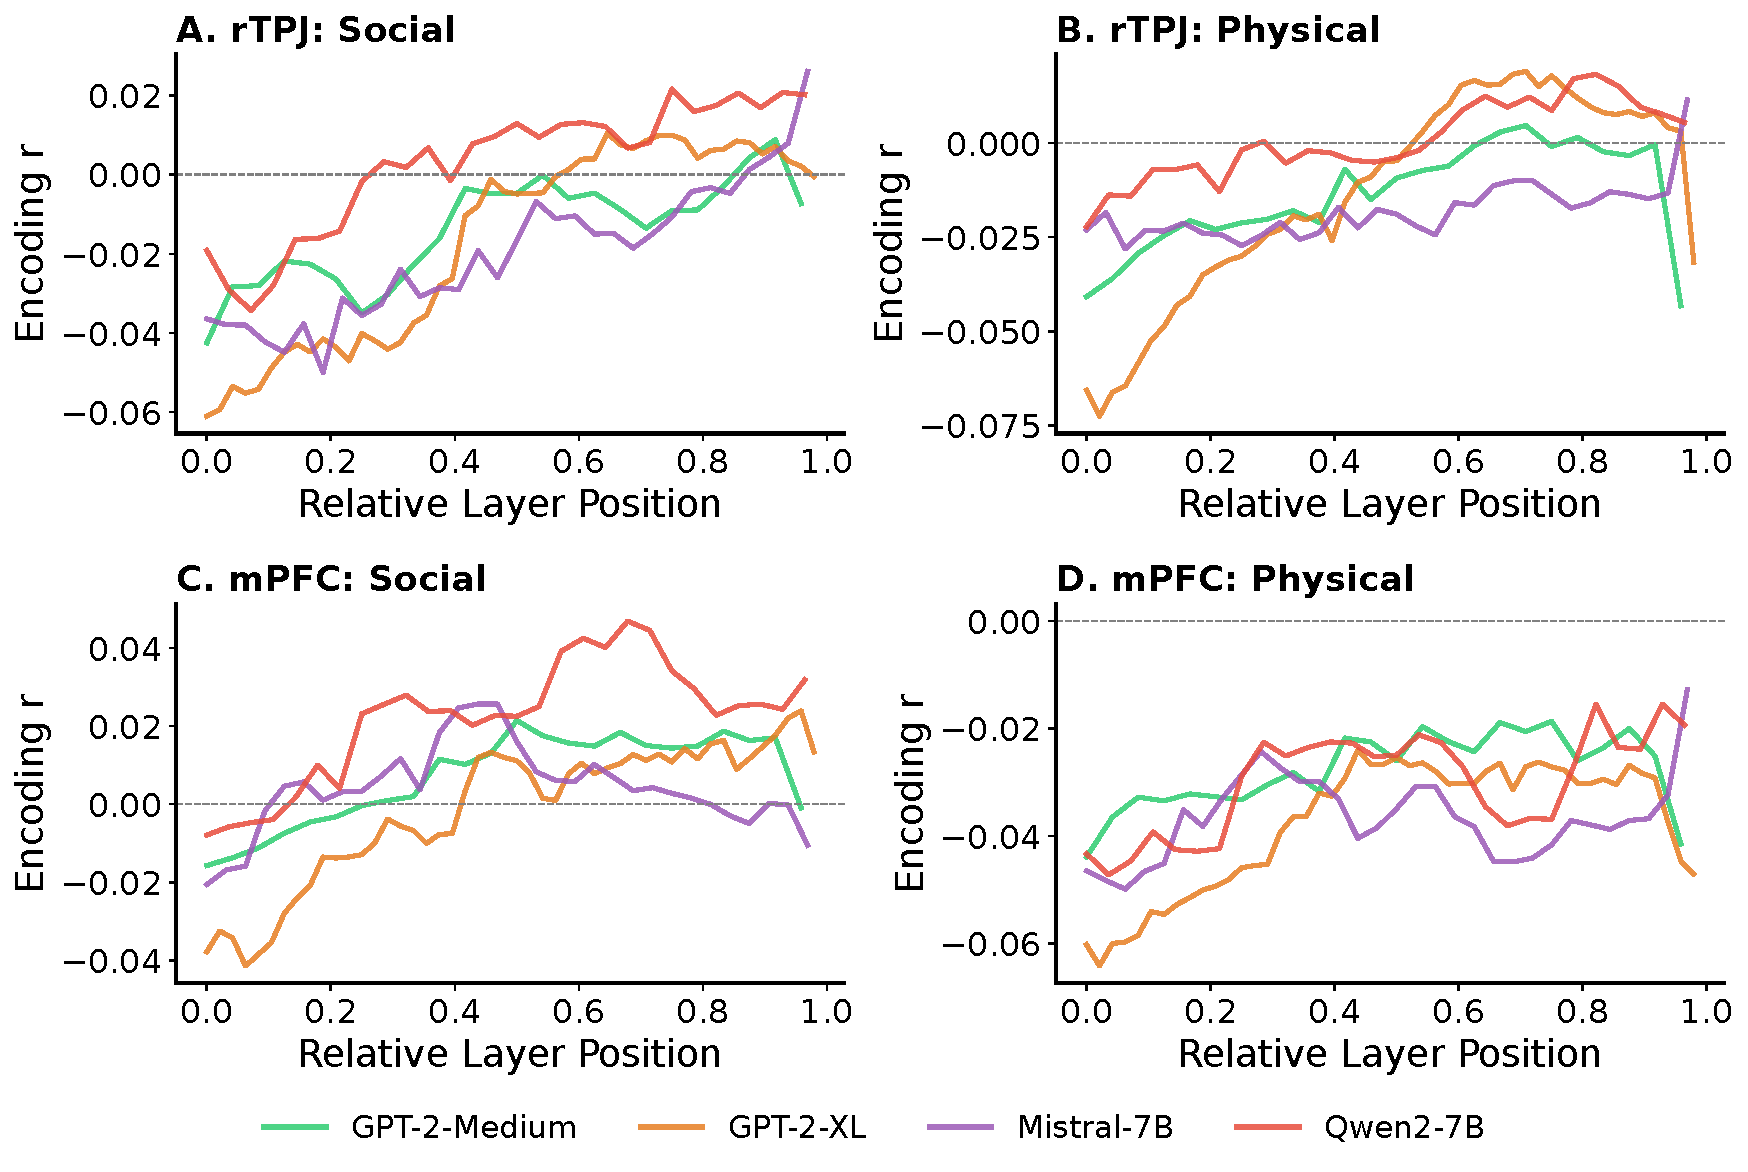
\includegraphics[width=\linewidth]{fig02_encoding_layers.pdf}
\caption{Layer-wise encoding $r$ for key ROIs. (A, B) rTPJ encoding for social and physical conditions. (C, D) mPFC encoding for social and physical conditions. Lines represent different models across normalized layer positions.}
\label{fig:encoding}
\end{figure}

\begin{figure}[t]
\centering
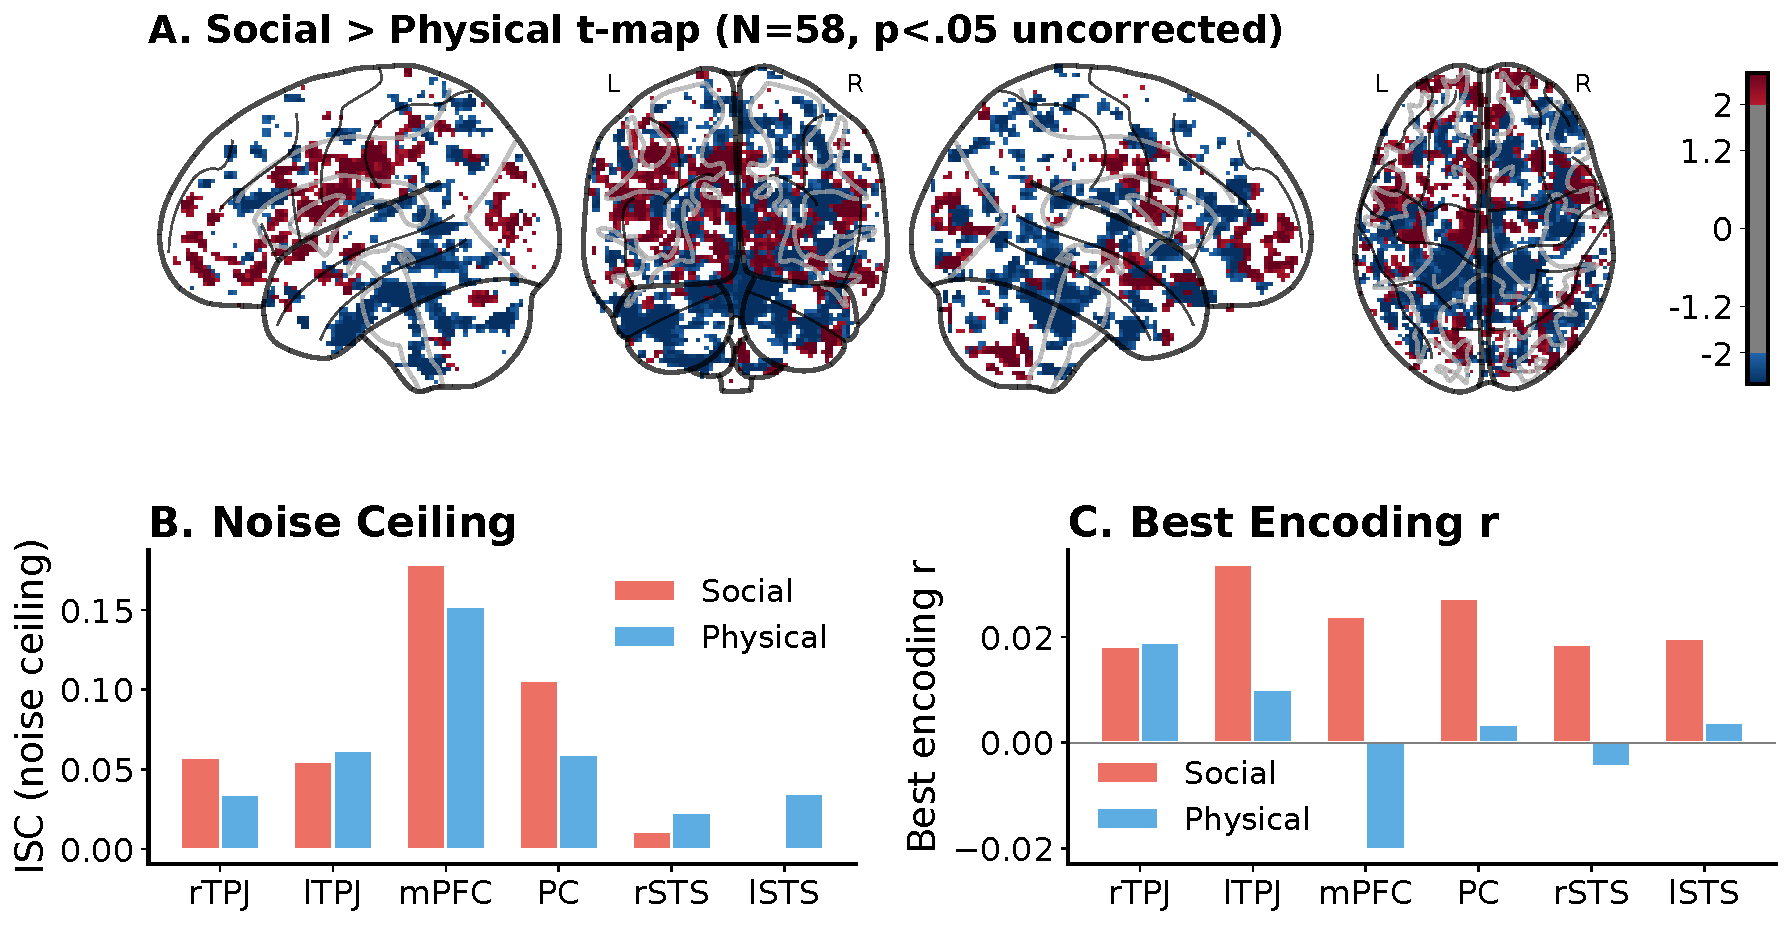
\includegraphics[width=\linewidth]{fig01_brain_encoding.pdf}
\caption{Brain ROI analysis. (A) Voxel-wise Social $>$ Physical $t$-map from a group-level paired $t$-test across 58 subjects on preprocessed whole-brain BOLD (thresholded at $|t|>2.0$, MNI152 brain mask applied). (B) Leave-one-out ISC per ROI and condition (conservative lower-bound noise ceiling). (C) Best encoding $r$ (across all layers) per ROI and condition.}
\label{fig:brain}
\end{figure}

\begin{figure}[t]
\centering
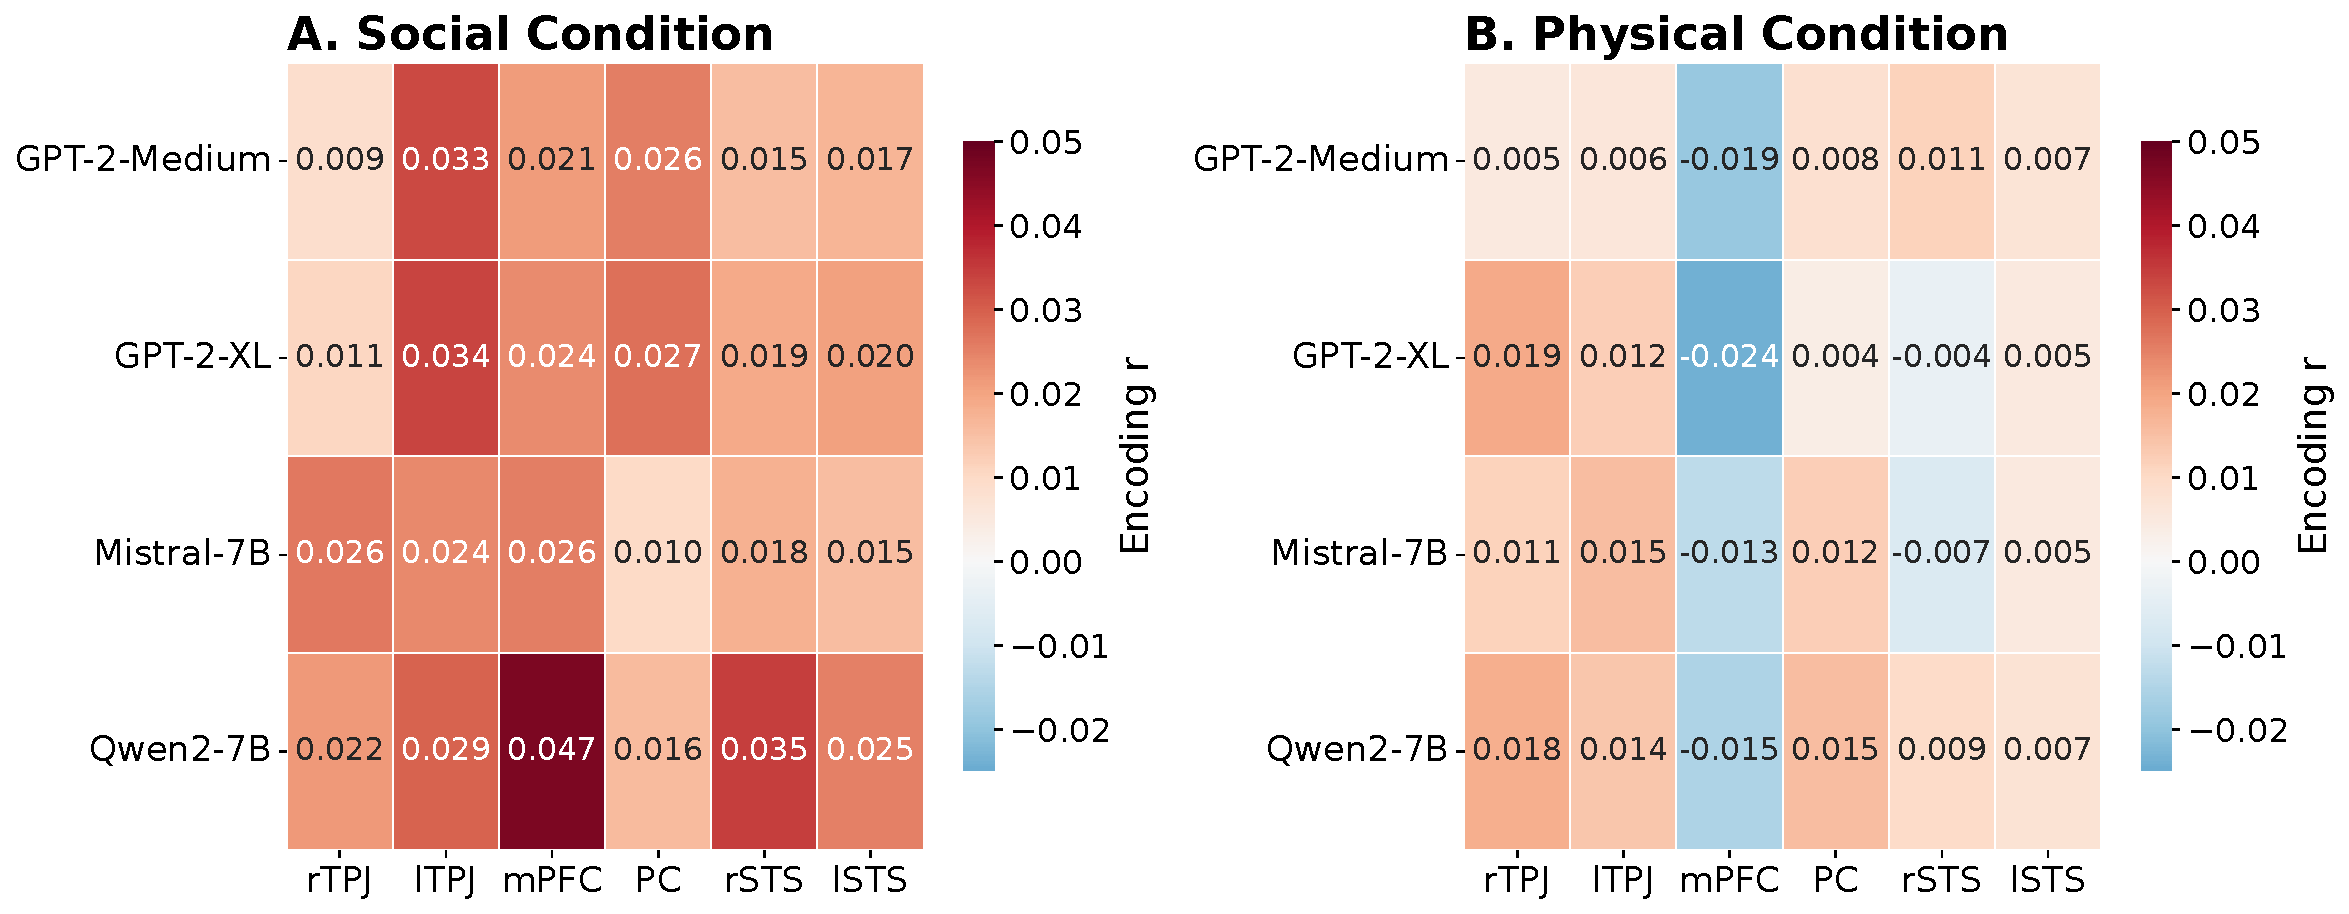
\includegraphics[width=\linewidth]{fig02_encoding_heatmap.pdf}
\caption{Best encoding $r$ per model (rows) and ROI (columns), shown separately for social (left) and physical (right) narratives. Color scale is diverging around zero; cells annotated with numeric $r$. Alignment is highest in mPFC for the social narrative but never exceeds $\sim0.05$.}
\label{fig:enc-heatmap}
\end{figure}


\subsection{Attention Sparsity: Architecture-Specific Patterns}
\label{sec:attention-sparsity-results}

Attention sparsity analysis found moderately concentrated attention across all models, with small but consistent condition differences (Fig.~\ref{fig:attention}). Across the three complementary metrics (Table~\ref{tab:sparsity}), Mistral-7B stood out with the highest Gini (0.768 social vs.\ 0.751 physical), the lowest entropy (0.499 social vs.\ 0.525 physical), and the highest top-5 concentration (0.568 social vs.\ 0.537 physical), indicating that roughly 57\% of the attention mass lands on just five tokens. In contrast, GPT-2-XL showed essentially uniform entropy (0.69) and the lowest top-5 concentration (0.32--0.36), consistent with its more diffuse attention pattern visible in the per-head heatmaps.

\begin{table}[t]
\centering
\caption{Attention sparsity by model and condition (S = social, P = physical).}
\label{tab:sparsity}
\vskip 0.05in
\small
\setlength{\tabcolsep}{3pt}
\begin{tabular}{lcccccc}
\toprule
 & \multicolumn{2}{c}{Gini} & \multicolumn{2}{c}{Entropy} & \multicolumn{2}{c}{Top-5} \\
Model & S & P & S & P & S & P \\
\midrule
GPT-2-Medium & 0.661 & 0.648 & 0.664 & 0.700 & 0.392 & 0.350 \\
GPT-2-XL     & 0.672 & 0.674 & 0.688 & 0.715 & 0.358 & 0.323 \\
Mistral-7B   & \textbf{0.768} & \textbf{0.751} & \textbf{0.499} & \textbf{0.525} & \textbf{0.568} & \textbf{0.537} \\
Qwen2-7B     & 0.673 & 0.652 & 0.671 & 0.703 & 0.381 & 0.344 \\
\bottomrule
\end{tabular}
\end{table}

All four models had higher sparsity for social than physical narratives by at least two of the three metrics. The differences are small in absolute terms (mean $\Delta$Gini 0.014--0.022, $\Delta$entropy $-0.027$ to $-0.036$) but highly consistent: paired across layers, social attention was sparser in 77--91\% of layers, with Wilcoxon $p \le 0.002$ and $|d_z| = 0.76$--$1.31$ for every model and metric (FDR-corrected), except the Gini coefficient of GPT-2-XL ($\Delta = -0.002$, $p = 0.69$), which is the one metric on which that model does not differ. Across all models and both conditions, the fraction of heads classified as ``sparse'' (Gini~$>0.5$) ranged from 78.6\% (GPT-2-Medium, physical) to 96.1\% (Mistral-7B, social), suggesting that the vast majority of heads implement some form of concentrated selection rather than diffuse averaging. The heatmaps (Fig.~\ref{fig:attention}) show more uniform sparsity across heads in GPT-2 and greater head-level variability in the 7B models.

\begin{figure}[t]
\centering
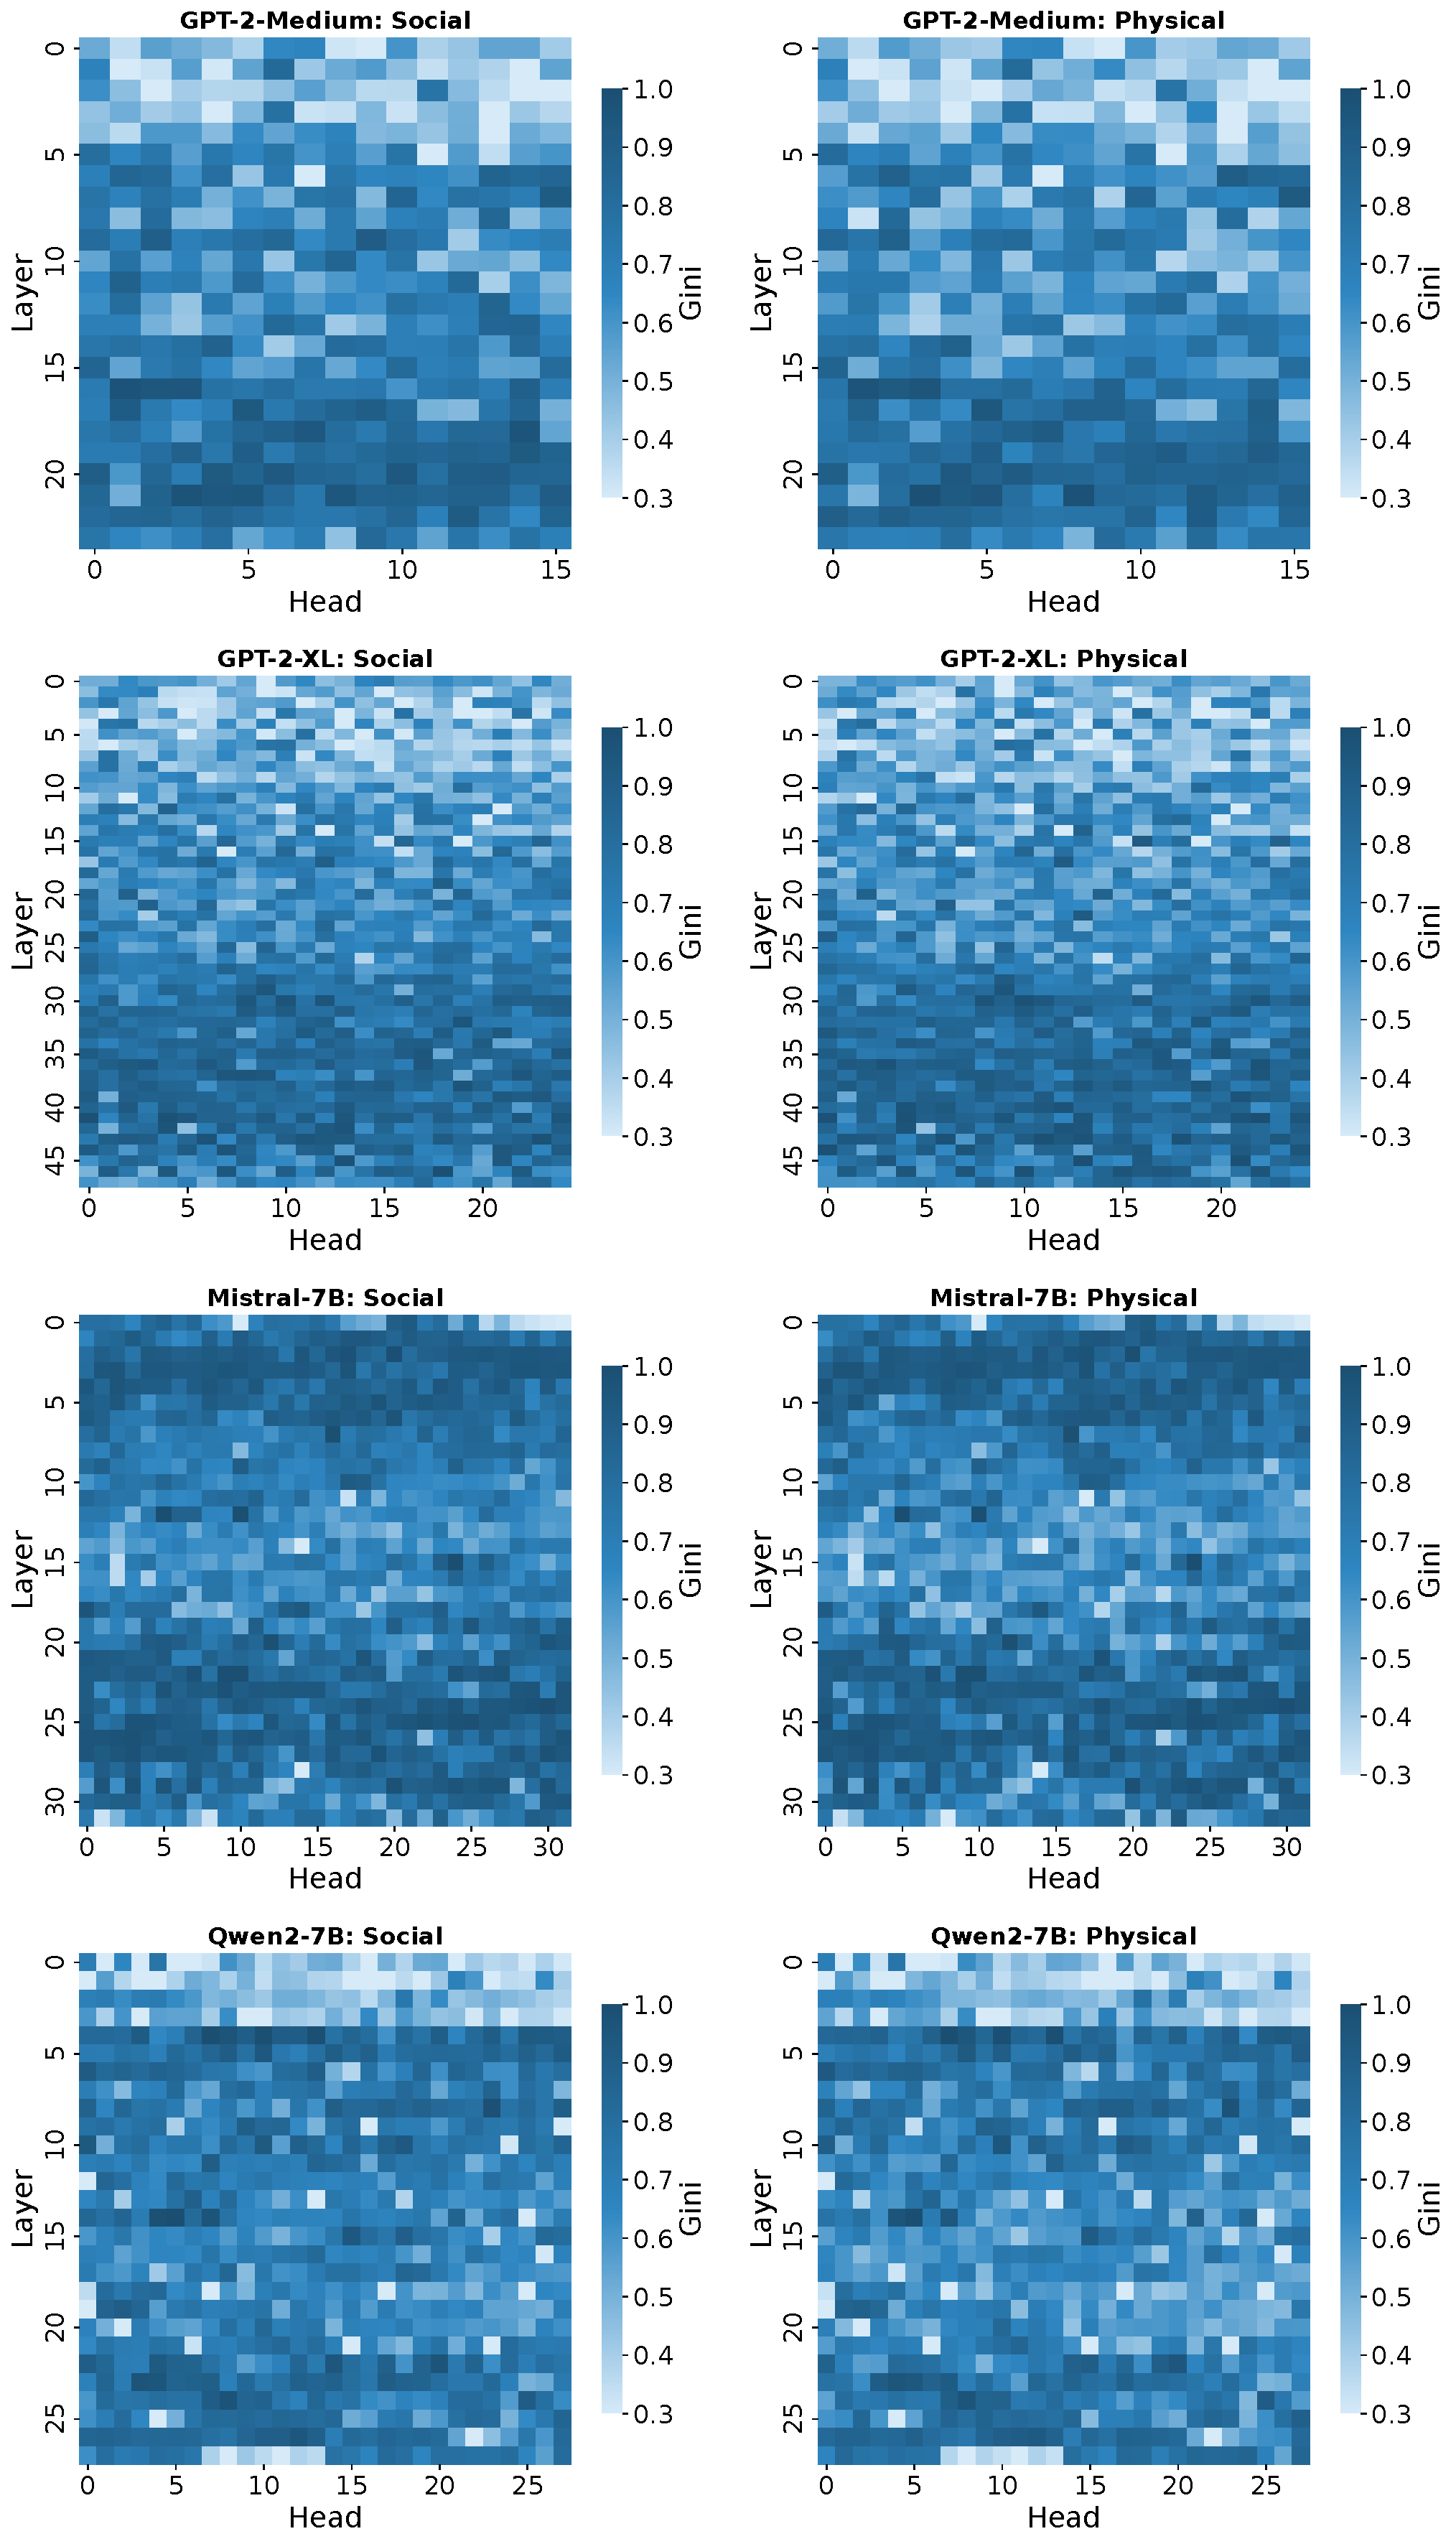
\includegraphics[width=0.9\linewidth]{fig05_attention_heatmaps.pdf}
\caption{Attention sparsity heatmaps showing Gini coefficient per layer (rows) and head (columns) for each model. Left: social condition; right: physical condition. Darker colors indicate higher sparsity.}
\label{fig:attention}
\end{figure}

\subsection{Causal Head Ablation: Large Single-Head Effects, Prompt-Dependent Circuits}
\label{sec:ablation}

On the original four prompts, zero-ablating individual attention heads showed that mental-state word prediction depends on a small subset of heads rather than being diffusely encoded (Table~\ref{tab:ablation}). For GPT-2-Medium, a single head (layer 6, head 1) carried a causal effect of $\Delta = 0.94$ logits, nearly 25\% of the model's baseline logit gap (3.81). The four models differed in their \textit{mean} ablation effect: near zero or slightly positive for GPT-2 and Mistral-7B, but \emph{negative} for Qwen2-7B ($-0.08$), i.e.\ ablating an average Qwen2 head \emph{improves} the target--control gap and only a small subset carries the positive signal. The top-5\% heads lay mostly in middle layers for GPT-2 and Mistral-7B (51--67\% of critical heads at 33--67\% relative depth) and were spread evenly across depth in Qwen2-7B.

The strongest heads of both 7B models sit in the very first layer (Mistral-7B layer 0, head 29; Qwen2-7B layer 0, head 10). Layer-0 heads commonly attend to position or to the beginning-of-sequence token, so their ablation disrupts processing structurally rather than semantically, and we do not interpret them as ToM-specific heads.

Extending the analysis to 19 prompts shows that the critical set is only partly stable. The critical heads from two random halves of the prompts overlapped with a Jaccard index of 0.18--0.30 for GPT-2 and Mistral-7B, 7--11 times the overlap expected by chance ($\approx 0.03$), but only 0.05 for Qwen2-7B; only 31--40\% of the heads that were critical on the original four prompts remained critical over all 19; and the per-prompt effect profiles were weakly correlated (mean pairwise Spearman $\rho = 0.02$--$0.09$). Part of the original result was driven by the \textit{father} prompt, whose baseline gap (11.8 logits in GPT-2-Medium) dominates the four-prompt average. The GPT-2-Medium head L6H1 remained the strongest head over all 19 prompts, and the layer-0 heads of the 7B models remained dominant. We therefore read the ablation as evidence that individual heads can have large, reproducible effects, but that the wider ``circuit'' depends substantially on the prompt; it should not be taken as a stable ToM module.

\begin{table}[t]
\centering
\caption{Causal head ablation. Base: mean target$-$control logit gap; Max: largest mean per-head drop (head); N crit.: heads $\geq$95th percentile. $J$: split-half Jaccard of the critical set over 19 prompts (chance $\approx 0.03$).}
\label{tab:ablation}
\vskip 0.05in
\footnotesize
\setlength{\tabcolsep}{2.5pt}
\begin{tabular}{lccccc}
\toprule
 & \multicolumn{3}{c}{Original 4 prompts} & \multicolumn{2}{c}{All 19 prompts} \\
\cmidrule(lr){2-4}\cmidrule(lr){5-6}
Model & Base & Max (head) & N crit. & Max (head) & $J$ \\
\midrule
GPT-2-Med.  & 3.81 & \textbf{0.94} (L6H1) & 20/384 & 0.18 (L6H1) & 0.30 \\
GPT-2-XL    & 2.33 & 0.22 (L24H19) & 60/1200 & 0.08 (L16H13) & 0.18 \\
Mistral-7B  & 3.90 & 0.52 (L0H29)$^\dagger$ & 55/1024 & 0.22 (L0H29)$^\dagger$ & 0.21 \\
Qwen2-7B    & 3.53 & 0.52 (L0H10)$^\dagger$ & 42/784 & 0.51 (L0H10)$^\dagger$ & 0.05 \\
\bottomrule
\multicolumn{6}{l}{$^\dagger$Layer-0 head; likely positional/BOS-driven (see text).}
\end{tabular}
\end{table}

\subsection{Robustness of the Weak Alignment}
\label{sec:robust}

We checked whether the weak alignment could be an artifact of four analysis choices.

\textit{Hemodynamic lag.} Re-running the full encoding analysis with feature lags of 0--6 TRs (0--9s) left the picture unchanged: the best $r$ across models and layers stayed at or below 0.061 in every ROI and at every lag. In mPFC it varied smoothly with lag (0.023, 0.034, 0.037, 0.047, 0.061, 0.039, 0.032 for lags 0--6), peaking at 4 TRs (6s), one TR after the lag used in the paper; in rTPJ the best $r$ was 0.026 at lag 3 and 0.031 at lag 4. A $\pm$1-TR change thus moves the best values by at most 0.014 and leaves the conclusion intact.

\textit{Encoder capacity.} At each model's best layer for every ROI and condition we compared the ridge encoder with three alternatives under the same cross-validation: ridge on 200 instead of 50 principal components, kernel ridge regression with an RBF kernel, and a one-hidden-layer MLP (64 units; mPFC and rTPJ only), with the hyperparameters of the nonlinear models tuned by contiguous-block cross-validation inside the training folds. Neither nonlinear encoder helped: kernel ridge scored below linear ridge in all 48 cells and the MLP in all 16 cells tested (best MLP $r = 0.029$). Using 200 components raised $r$ in 21 of 48 cells, but no change survived FDR correction (smallest $q = 0.19$) and the best value remained 0.044. The weak alignment is therefore not a limitation of the linear read-out.

\textit{ROI size.} Re-extracting all six ROIs as 8mm (257 voxels) and 6mm (123 voxels) spheres and repeating the encoding analysis did not raise alignment. The best value overall was $r = 0.051$ (Qwen2-7B, mPFC, 6mm) against 0.047 at the original radius; mPFC changed by at most 0.005 for every model and condition, and TPJ values fell (e.g.\ Mistral-7B rTPJ from 0.026 to 0.009 at 6mm), in line with a drop in ISC as fewer voxels are averaged (mPFC 0.184 $\rightarrow$ 0.141). Spatial imprecision of the spheres therefore does not explain the weak alignment.

\textit{GPT-2 context truncation.} Dropping the story TRs beyond the GPT-2 context window (31 social and 44 physical TRs, \S\ref{sec:methods:features}) changed the best GPT-2 encoding per ROI by at most 0.03, in both directions and without a systematic trend, and no value exceeded 0.05; the nearest-TR filling therefore does not account for the GPT-2 results, and the GPT-2 and 7B numbers can be compared.

\section{Discussion}

\subsection{Behavioral Success Without Representational Alignment}

Our findings expose a dissociation between behavioral competence and neural alignment. 7B transformer models solve explicit ToM items at 75--83\% accuracy, and all four models we tested readily distinguish social from physical descriptions of identical visual events (89--98\% probing accuracy), yet their internal representations align only weakly with human brain activity during the same task (best $r \le 0.05$, and not reliably above zero after correction). Transformers and brains may thus solve similar ToM-related tasks through fundamentally different computational strategies. This cautions against using behavioral ToM benchmarks as evidence for human-like social understanding in AI systems: systems that appear to understand social situations may rely on different, and potentially brittle, computational strategies.

The weak encoding performance should be interpreted relative to the noise ceiling. With ISC-based upper bounds of 0.16--0.25, the best encoding correlations ($r = 0.026$--$0.047$) achieve roughly 16--21\% of the ceiling. This is substantially lower than encoding results reported for language comprehension, where models can explain 20--50\% of the neural variance \cite{schrimpf2021neural, caucheteux2022brains, goldstein2022shared}. The gap suggests that social cognition involves computational principles not well captured by current language model architectures.

\subsection{Early Representational Divergence}

In the 7B models the social--physical distinction is near its peak by layer 4, and a bag-of-words probe alone reaches 74\%, both pointing to a substantial lexical component. The models may separate the narratives by vocabulary (mental-state words vs.\ geometric terms) rather than by mentalizing computations, which would explain why classification succeeds while alignment with the brain's higher-order social inference remains weak.

\subsection{Model Scale and Alignment Trends}

The four models span roughly 20$\times$ in parameter count (355M to 7B), providing a small but informative window into scaling effects. Behavioral ToM accuracy tracks parameter count cleanly: 7B models (83.3\% and 75.0\% overall) nearly double the performance of the GPT-2 variants ($\sim$50\%). Brain-model encoding alignment, however, shows no such monotonic trend: Qwen2-7B reaches the highest mPFC correlation ($r = 0.047$), but Mistral-7B, of the same size, does not exceed the GPT-2 models there ($r = 0.026$ vs.\ 0.021--0.024), and in lTPJ and precuneus the best values come from GPT-2-XL and GPT-2-Medium. Parameter count thus improves task performance more reliably than representational plausibility. It also constrains the interpretation of larger models (e.g., GPT-4) that solve textbook ToM tasks \cite{kosinski2024evaluating, strachan2024testing}: impressive behavioral performance need not imply brain-like mechanisms.

Why would scale buy behavior but not alignment? First, next-token prediction rewards whatever statistics predict the continuation, and classic ToM items are short, formulaic narratives whose answers are often recoverable from co-occurrence cues (``put the ball in the basket \ldots\ looks in the'' $\rightarrow$ \emph{basket}); larger models capture such cues more reliably, and published items and their variants are likely present in pretraining data \cite{ullman2023large, shapira2024clever}. Second, the behavioral test scores a single forced-choice token, whereas encoding asks the whole representation to track a social situation that evolves over minutes; a model can favor the right answer word without maintaining a persistent model of the agents' beliefs. Third, human mentalizing is shaped by embodiment, interaction and the need to predict other agents, none of which enters text-only pretraining. Scale thus mainly sharpens heuristics that already work for the benchmark, consistent with the flat alignment curve and with the fragility of ToM performance under small perturbations \cite{ullman2023large}.

\subsection{Layer Trajectories and the Missing Middle}

In language comprehension studies, encoding peaks typically occur in the \textit{middle} layers of transformer models (around 50--70\% depth), reflecting a hierarchy from lexical to compositional to semantic processing \cite{caucheteux2022brains, schrimpf2021neural}. Our data show an inconsistent picture: best-encoding layers for mPFC range from layer 15 of Mistral-7B (47\% depth) and layer 12 of GPT-2-Medium (50\%) to layer 19 of Qwen2-7B (68\%) and layer 46 of GPT-2-XL (96\%), while probing accuracy in the 7B models peaks at layer 4. That probing and brain-encoding peaks do not co-locate on the layer axis suggests that the features the probe relies on (likely lexical) and the features the brain activity reflects (presumably integrative) live in different parts of the network. The causal heads tell the same story. Their centre of mass lies at 36--44\% relative depth in every model, whereas encoding peaks at 47--97\%; across layers, the number of critical heads is not consistently related to encoding $r$ (Spearman $\rho$ from $-0.54$ to $0.36$ over models and ROIs, mPFC and rTPJ), and encoding at the layers that host critical heads is no higher than the layer average (e.g.\ 0.020 vs.\ 0.022 in Qwen2-7B mPFC). The components that are causally necessary for mental-state word prediction thus sit where the models are no more brain-like than anywhere else, which links the behavioral and alignment results into one picture: the machinery that produces the right mental-state word is not the part of the network that tracks the brain's response to the story. This motivates future work on intermediate representations between linear-probe accessible features and higher-order social inference.

\subsection{Limitations and Future Directions}

Several limitations should be noted. First, we used atlas-based ROIs rather than individually localized regions; smaller spheres did not change the result (\S\ref{sec:robust}), but individual functional localization could still sharpen the ROI signal. Second, the BOLD data were not processed through fMRIPrep; the significant ISC in mPFC, precuneus and TPJ shows that our preprocessing preserves a reliable stimulus-locked signal there, but the near-zero ISC in STS means that alignment in STS is effectively untestable with these data. Third, the social advantage in encoding is a consistent trend that does not survive correction; a larger stimulus set with more social/physical pairs would be needed to establish or refute it. Fourth, only four of six planned models could be analyzed due to compatibility issues. Fifth, our behavioral ToM benchmark (24 items) is small; larger, contamination-controlled benchmarks would strengthen the scaling conclusions. Sixth, even with 19 prompts the critical-head set is only partly stable, and the dominant layer-0 heads of the 7B models are likely structural rather than semantic, so the ablation results characterize prompt-specific rather than general ToM circuitry. Future work should employ fMRIPrep-processed data with individually localized ROIs, larger and more diverse behavioral and ablation sets, and larger model families including multimodal models that can process visual ToM stimuli directly.

\subsection{Conclusion}

This study provides modality-matched evidence that 7B-scale transformer language models solve classic Theory of Mind items at 75--83\% accuracy, and that the hidden states of all four models we tested separate social from physical narratives (89--98\% probing accuracy, well above a 74\% lexical baseline). Yet the models' internal states align only weakly with the human brain's social cognition network: the best encoding reaches $r = 0.047$ (about 19\% of the noise-ceiling upper bound), does not survive correction across cells, and does not improve with other hemodynamic lags, nonlinear encoders or smaller ROIs. Causal head ablation finds individual heads with large effects on mental-state word prediction, but a critical-head set that depends substantially on the prompt and sits in layers where alignment is no better than elsewhere. The dissociation between behavioral success and representational alignment suggests that current LLMs achieve ToM-like performance through computational strategies different from human mentalizing. For cognitive science, these results indicate that behavioral similarity should not be taken as evidence for mechanistic similarity, a principle with broad implications for evaluating AI systems' cognitive capabilities.

\section*{Acknowledgment}

Data were provided by the Narratives collection \cite{nastase2021narratives} (OpenNeuro ds002345). We thank the Princeton Neuroscience Institute for data collection and sharing.

\textit{AI-generated content disclosure.} For the camera-ready version the authors used Claude (Claude Opus 5.5, Anthropic) to (i) correct the word-to-TR alignment code (\S\ref{sec:methods:features}) and write the scripts for the analyses added in response to the reviewers, (ii) draft parts of the revised Methods, Results (\S\ref{sec:ablation}, \S\ref{sec:robust} and the encoding and probing results) and Discussion, and (iii) edit language throughout. The authors ran and checked all code and results and revised all text, and take full responsibility for the content.

\begin{thebibliography}{00}

\bibitem{frith2006neural} C. D. Frith and U. Frith, ``The neural basis of mentalizing,'' \textit{Neuron}, vol. 50, no. 4, pp. 531--534, 2006.

\bibitem{saxe2013people} R. Saxe, ``The new puzzle of Theory of Mind development,'' in \textit{Navigating the Social World}, A. Banaji and S. Gelman, Eds. Oxford Univ. Press, 2013.

\bibitem{soutschek2025causal} A. Soutschek et al., ``Causal role of the temporo-parietal junction in Theory of Mind,'' \textit{Neurosci. Biobehav. Rev.}, 2025.

\bibitem{amodio2006meeting} D. M. Amodio and C. D. Frith, ``Meeting of minds: the medial frontal cortex and social cognition,'' \textit{Nat. Rev. Neurosci.}, vol. 7, pp. 268--277, 2006.

\bibitem{allison2000social} T. Allison, A. Puce, and G. McCarthy, ``Social perception from visual cues: role of the STS region,'' \textit{Trends Cogn. Sci.}, vol. 4, no. 7, pp. 267--278, 2000.

\bibitem{mar2011neural} R. A. Mar, ``The neural bases of social cognition and story comprehension,'' \textit{Annu. Rev. Psychol.}, vol. 62, pp. 103--134, 2011.

\bibitem{kosinski2024evaluating} M. Kosinski, ``Evaluating large language models in Theory of Mind tasks,'' \textit{arXiv:2302.02083}, 2024.

\bibitem{ullman2023large} T. Ullman, ``Large language models fail on trivial alterations to Theory-of-Mind tasks,'' \textit{arXiv:2302.08399}, 2023.

\bibitem{shapira2024clever} N. Shapira et al., ``Clever Hans or neural Theory of Mind?,'' in \textit{Proc. EACL}, 2024.

\bibitem{strachan2024testing} J. W. A. Strachan et al., ``Testing Theory of Mind in large language models and humans,'' \textit{Nat. Hum. Behav.}, vol. 8, pp. 1285--1295, 2024.

\bibitem{chen2024tombench} Z. Chen et al., ``ToMBench: Benchmarking Theory of Mind in large language models,'' in \textit{Proc. ACL}, 2024.

\bibitem{wilf2024think} N. Wilf et al., ``Think twice: Perspective-taking improves large language models' Theory-of-Mind capabilities,'' in \textit{Proc. ACL}, 2024.

\bibitem{sap2022neural} M. Sap et al., ``Neural Theory-of-Mind? On the limits of social intelligence in large LMs,'' in \textit{Proc. EMNLP}, 2022.

\bibitem{marcus2023large} G. Marcus, ``Large language models and the limits of understanding,'' \textit{AI Mag.}, 2023.

\bibitem{ji2026captain} B. Ji et al., ``CAPTAIN: a multimodal foundation model pretrained on co-assayed single-cell RNA and protein,'' \textit{Nat. Commun.}, vol. 17, 6161, 2026, doi: 10.1038/s41467-026-72882-y.

\bibitem{ji2024spaccc} B. Ji et al., ``SpaCCC: Large language model-based cell-cell communication inference for spatially resolved transcriptomic data,'' \textit{Big Data Min. Anal.}, vol. 7, no. 4, pp. 1129--1147, 2024, doi: 10.26599/BDMA.2024.9020056.

\bibitem{ji2024scdca} B. Ji et al., ``scDCA: deciphering the dominant cell communication assembly of downstream functional events from single-cell RNA-seq data,'' \textit{Brief. Bioinform.}, vol. 26, no. 1, bbae663, 2025, doi: 10.1093/bib/bbae663.

\bibitem{khaligh2014deep} S. A. Khaligh-Razavi and N. Kriegeskorte, ``Deep supervised, but not unsupervised, models may explain IT cortical representation,'' \textit{PLoS Comput. Biol.}, vol. 10, e1003915, 2014.

\bibitem{schrimpf2021neural} M. Schrimpf et al., ``The neural architecture of language: Integrative modeling converges on predictive processing,'' \textit{Proc. Natl. Acad. Sci.}, vol. 118, e2105646118, 2021.

\bibitem{caucheteux2022brains} C. Caucheteux and J.-R. King, ``Brains and algorithms partially converge in natural language processing,'' \textit{Commun. Biol.}, vol. 5, 134, 2022.

\bibitem{goldstein2022shared} A. Goldstein et al., ``Shared computational principles for language processing in humans and deep language models,'' \textit{Nat. Neurosci.}, vol. 25, pp. 369--380, 2022.

\bibitem{nastase2021narratives} S. A. Nastase et al., ``The `Narratives' fMRI dataset for evaluating models of naturalistic language comprehension,'' \textit{Sci. Data}, vol. 8, 250, 2021.

\bibitem{schurz2014fractionating} M. Schurz et al., ``Fractionating Theory of Mind: A meta-analysis of functional brain imaging studies,'' \textit{Neurosci. Biobehav. Rev.}, vol. 42, pp. 9--34, 2014.

\bibitem{kriegeskorte2008representational} N. Kriegeskorte, M. Mur, and P. Bandettini, ``Representational similarity analysis,'' \textit{Front. Syst. Neurosci.}, vol. 2, 4, 2008.

\bibitem{elhage2021mathematical} N. Elhage et al., ``A mathematical framework for transformer circuits,'' \textit{Transformer Circuits Thread}, Anthropic, 2021.

\bibitem{wang2022interpretability} K. Wang et al., ``Interpretability in the wild: a circuit for indirect object identification in GPT-2 small,'' in \textit{Proc. ICLR}, 2022.

\bibitem{conmy2023towards} A. Conmy et al., ``Towards automated circuit discovery for mechanistic interpretability,'' in \textit{Proc. NeurIPS}, 2023.

\bibitem{wolf2020transformers} T. Wolf et al., ``Transformers: State-of-the-art natural language processing,'' in \textit{Proc. EMNLP: System Demonstrations}, 2020, pp. 38--45.

\bibitem{hoyer2004non} P. O. Hoyer, ``Non-negative matrix factorization with sparseness constraints,'' \textit{J. Mach. Learn. Res.}, vol. 5, pp. 1457--1469, 2004.

\end{thebibliography}

\end{document}
